\documentclass{standalone}
\usepackage{tikz}
\usetikzlibrary{patterns, positioning}
\usepackage[sfdefault]{ClearSans} %% option 'sfdefault' activates Clear Sans as the default text font
\usepackage[T1]{fontenc}

\begin{document}
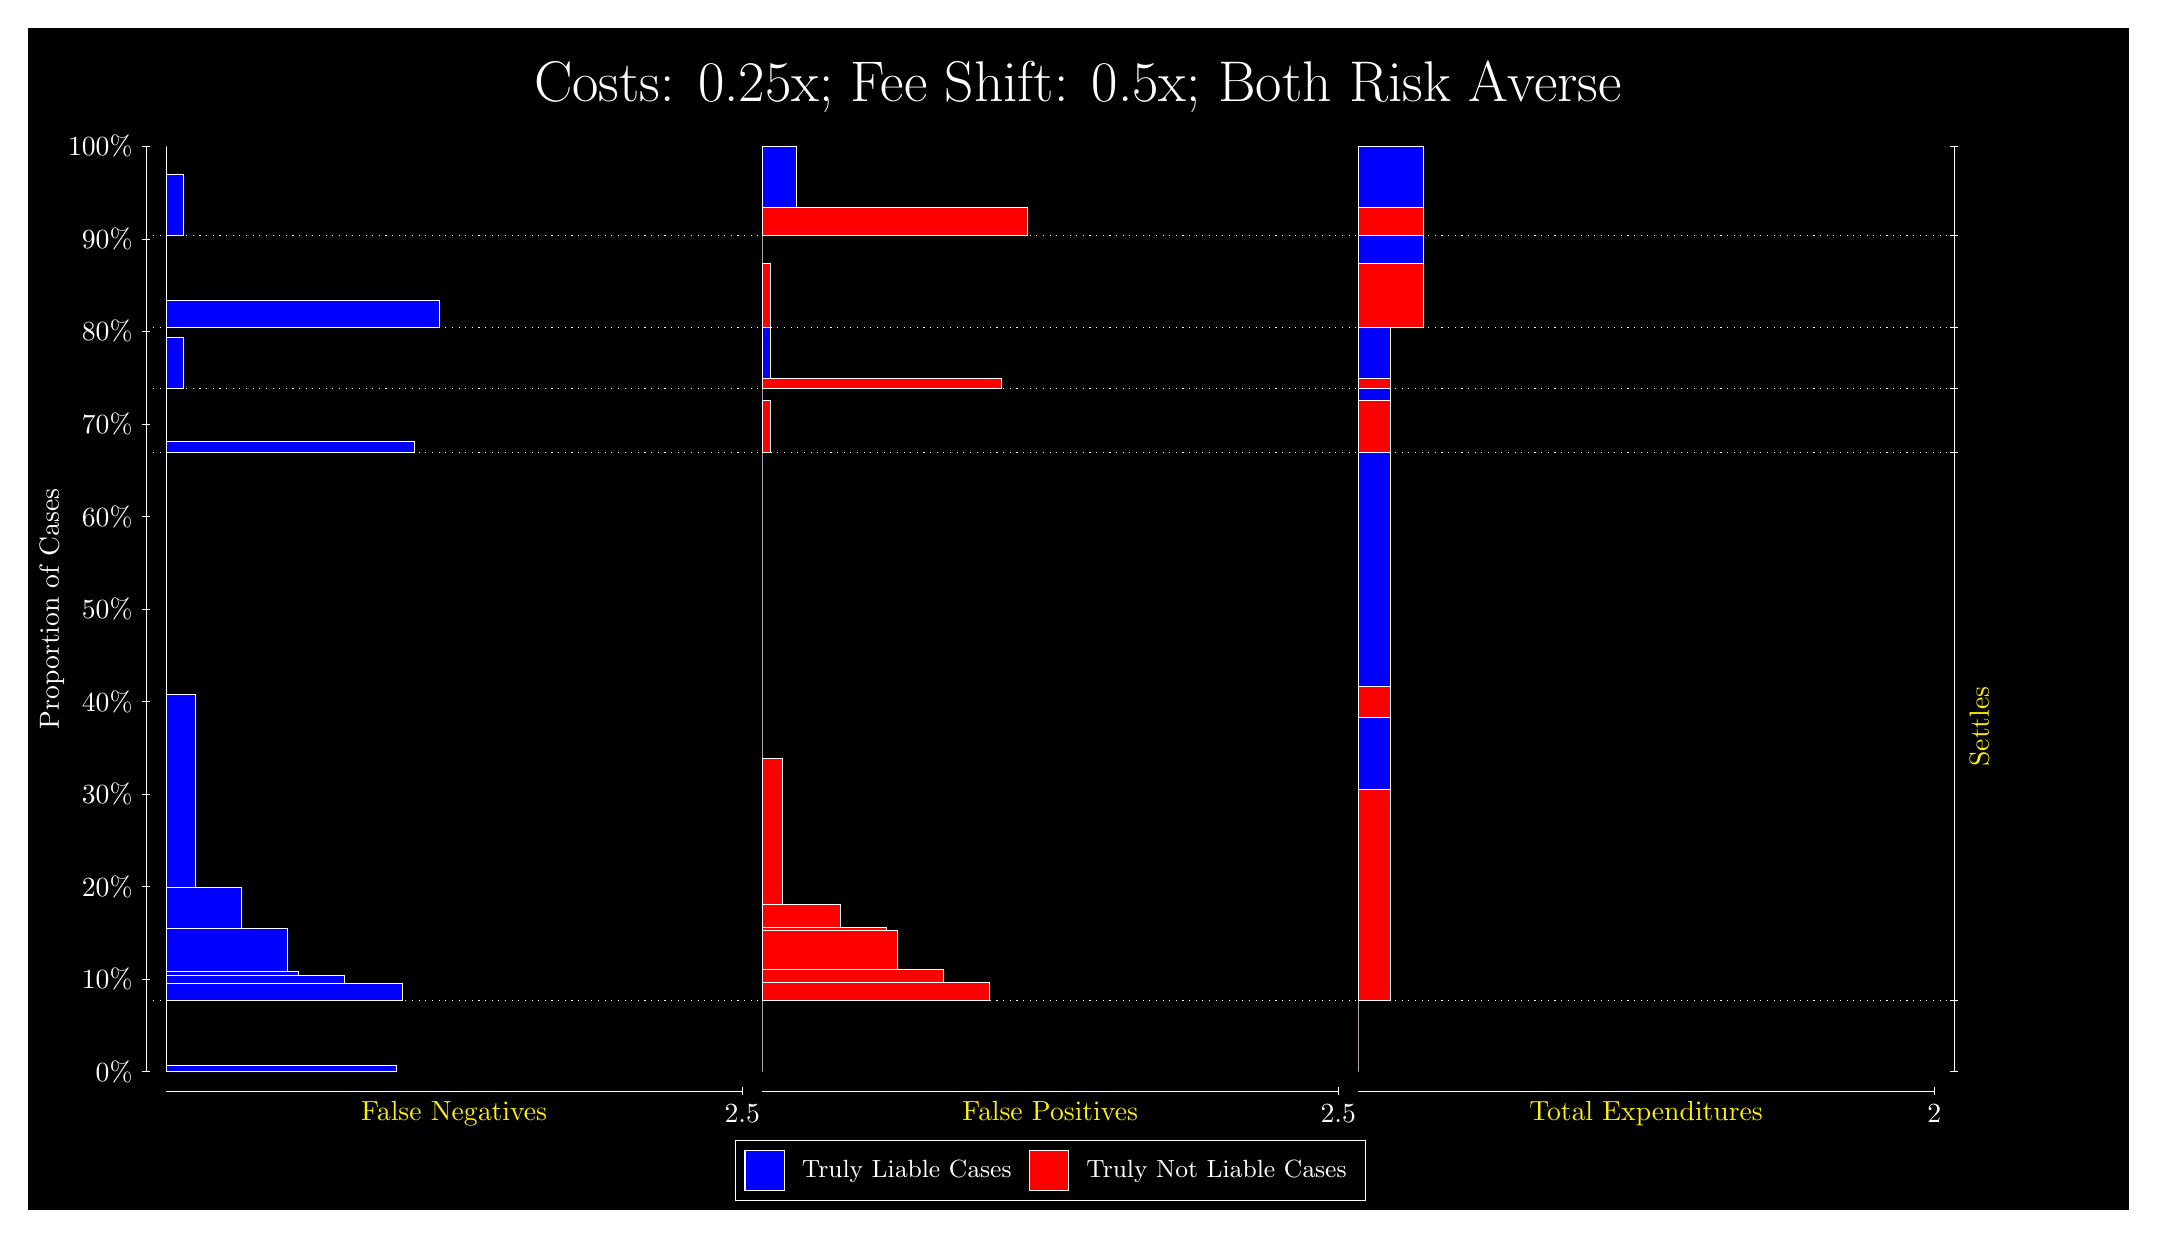
\begin{tikzpicture}
\draw[fill=black] (0,0) rectangle (26.667,15);
\draw[text=white] (0,13.5) rectangle (26.667,15) node[midway] {\huge Costs: 0.25x; Fee Shift: 0.5x; Both Risk Averse};
\draw[white, very thin] (1.5,1.75) -- (1.5,13.5);
\node[rotate=90, text=white, anchor=center] at (0.3, 7.625) {Proportion of Cases};
\draw[white, very thin] (1.45,1.75) -- (1.55,1.75);
\node[text=white, anchor=east] at (1.45, 1.75) {0\%};
\draw[white, very thin] (1.45,2.925) -- (1.55,2.925);
\node[text=white, anchor=east] at (1.45, 2.925) {10\%};
\draw[white, very thin] (1.45,4.1) -- (1.55,4.1);
\node[text=white, anchor=east] at (1.45, 4.1) {20\%};
\draw[white, very thin] (1.45,5.275) -- (1.55,5.275);
\node[text=white, anchor=east] at (1.45, 5.275) {30\%};
\draw[white, very thin] (1.45,6.45) -- (1.55,6.45);
\node[text=white, anchor=east] at (1.45, 6.45) {40\%};
\draw[white, very thin] (1.45,7.625) -- (1.55,7.625);
\node[text=white, anchor=east] at (1.45, 7.625) {50\%};
\draw[white, very thin] (1.45,8.8) -- (1.55,8.8);
\node[text=white, anchor=east] at (1.45, 8.8) {60\%};
\draw[white, very thin] (1.45,9.975) -- (1.55,9.975);
\node[text=white, anchor=east] at (1.45, 9.975) {70\%};
\draw[white, very thin] (1.45,11.15) -- (1.55,11.15);
\node[text=white, anchor=east] at (1.45, 11.15) {80\%};
\draw[white, very thin] (1.45,12.325) -- (1.55,12.325);
\node[text=white, anchor=east] at (1.45, 12.325) {90\%};
\draw[white, very thin] (1.45,13.5) -- (1.55,13.5);
\node[text=white, anchor=east] at (1.45, 13.5) {100\%};

\draw[white, very thin] (24.457,1.75) -- (24.457,13.5);
\draw[white, very thin] (24.407,1.75) -- (24.507,1.75);
\node[anchor=west] at (24.407, 1.75) {};
\draw[white, very thin] (24.407,2.6525) -- (24.507,2.6525);
\node[anchor=west] at (24.407, 2.6525) {};
\draw[white, very thin] (24.407,9.6128) -- (24.507,9.6128);
\node[anchor=west] at (24.407, 9.6128) {};
\draw[white, very thin] (24.407,10.422) -- (24.507,10.422);
\node[anchor=west] at (24.407, 10.422) {};
\draw[white, very thin] (24.407,11.197) -- (24.507,11.197);
\node[anchor=west] at (24.407, 11.197) {};
\draw[white, very thin] (24.407,12.371) -- (24.507,12.371);
\node[anchor=west] at (24.407, 12.371) {};
\draw[white, very thin] (24.407,13.5) -- (24.507,13.5);
\node[anchor=west] at (24.407, 13.5) {};

\draw[white, very thin, fill=blue] (1.75,1.75) rectangle (4.6775,1.8231);
\draw[white, very thin, fill=red] (1.75,1.8231) rectangle (1.75,2.6525);
\draw[white, very thin, fill=blue] (1.75,2.6525) rectangle (4.7507,2.8674);
\draw[white, very thin, fill=blue] (1.75,2.8674) rectangle (4.0188,2.9779);
\draw[white, very thin, fill=blue] (1.75,2.9779) rectangle (3.4333,3.0259);
\draw[white, very thin, fill=blue] (1.75,3.0259) rectangle (3.287,3.5675);
\draw[white, very thin, fill=blue] (1.75,3.5675) rectangle (2.7015,4.0922);
\draw[white, very thin, fill=blue] (1.75,4.0922) rectangle (2.1159,6.5356);
\draw[white, very thin, fill=red] (1.75,6.5356) rectangle (1.75,9.6128);
\draw[white, very thin, fill=blue] (1.75,9.6128) rectangle (4.8971,9.7548);
\draw[white, very thin, fill=red] (1.75,9.7548) rectangle (1.75,10.422);
\draw[white, very thin, fill=blue] (1.75,10.422) rectangle (1.9696,11.07);
\draw[white, very thin, fill=red] (1.75,11.07) rectangle (1.75,11.197);
\draw[white, very thin, fill=blue] (1.75,11.197) rectangle (5.2265,11.549);
\draw[white, very thin, fill=red] (1.75,11.549) rectangle (1.75,12.371);
\draw[white, very thin, fill=blue] (1.75,12.371) rectangle (1.9696,13.148);
\draw[white, very thin, fill=red] (1.75,13.148) rectangle (1.75,13.5);
\draw[white, very thin, fill=red] (9.3189,1.75) rectangle (9.3189,2.5794);
\draw[white, very thin, fill=blue] (9.3189,2.5794) rectangle (9.3189,2.6525);
\draw[white, very thin, fill=red] (9.3189,2.6525) rectangle (12.21,2.8863);
\draw[white, very thin, fill=red] (9.3189,2.8863) rectangle (11.624,3.0468);
\draw[white, very thin, fill=red] (9.3189,3.0468) rectangle (11.039,3.5387);
\draw[white, very thin, fill=red] (9.3189,3.5387) rectangle (10.892,3.5833);
\draw[white, very thin, fill=red] (9.3189,3.5833) rectangle (10.307,3.8762);
\draw[white, very thin, fill=red] (9.3189,3.8762) rectangle (9.575,5.7297);
\draw[white, very thin, fill=blue] (9.3189,5.7297) rectangle (9.3189,9.6128);
\draw[white, very thin, fill=red] (9.3189,9.6128) rectangle (9.4287,10.28);
\draw[white, very thin, fill=blue] (9.3189,10.28) rectangle (9.3189,10.422);
\draw[white, very thin, fill=red] (9.3189,10.422) rectangle (12.356,10.549);
\draw[white, very thin, fill=blue] (9.3189,10.549) rectangle (9.4287,11.197);
\draw[white, very thin, fill=red] (9.3189,11.197) rectangle (9.4287,12.018);
\draw[white, very thin, fill=blue] (9.3189,12.018) rectangle (9.3189,12.371);
\draw[white, very thin, fill=red] (9.3189,12.371) rectangle (12.686,12.723);
\draw[white, very thin, fill=blue] (9.3189,12.723) rectangle (9.758,13.5);
\draw[white, very thin, fill=red] (16.888,1.75) rectangle (16.888,2.5794);
\draw[white, very thin, fill=blue] (16.888,2.5794) rectangle (16.888,2.6525);
\draw[white, very thin, fill=red] (16.888,2.6525) rectangle (17.299,5.3353);
\draw[white, very thin, fill=blue] (16.888,5.3353) rectangle (17.299,6.2503);
\draw[white, very thin, fill=red] (16.888,6.2503) rectangle (17.299,6.6447);
\draw[white, very thin, fill=blue] (16.888,6.6447) rectangle (17.299,9.6128);
\draw[white, very thin, fill=red] (16.888,9.6128) rectangle (17.299,10.28);
\draw[white, very thin, fill=blue] (16.888,10.28) rectangle (17.299,10.422);
\draw[white, very thin, fill=red] (16.888,10.422) rectangle (17.299,10.549);
\draw[white, very thin, fill=blue] (16.888,10.549) rectangle (17.299,11.197);
\draw[white, very thin, fill=red] (16.888,11.197) rectangle (17.711,12.018);
\draw[white, very thin, fill=blue] (16.888,12.018) rectangle (17.711,12.371);
\draw[white, very thin, fill=red] (16.888,12.371) rectangle (17.711,12.723);
\draw[white, very thin, fill=blue] (16.888,12.723) rectangle (17.711,13.5);
\draw[white, dotted] (1.5,2.6525) -- (24.457,2.6525);
\draw[white, dotted] (1.5,9.6128) -- (24.457,9.6128);
\draw[white, dotted] (1.5,10.422) -- (24.457,10.422);
\draw[white, dotted] (1.5,11.197) -- (24.457,11.197);
\draw[white, dotted] (1.5,12.371) -- (24.457,12.371);
\draw[white, very thin] (1.75,1.5) -- (9.0689,1.5);
\node[text=yellow, anchor=north] at (5.4094, 1.5) {False Negatives};
\draw[white, very thin] (9.0689,1.45) -- (9.0689,1.55);
\node[text=white, anchor=north] at (9.0689, 1.45) {2.5};

\draw[white, very thin] (9.3189,1.5) -- (16.638,1.5);
\node[text=yellow, anchor=north] at (12.978, 1.5) {False Positives};
\draw[white, very thin] (16.638,1.45) -- (16.638,1.55);
\node[text=white, anchor=north] at (16.638, 1.45) {2.5};

\draw[white, very thin] (16.888,1.5) -- (24.207,1.5);
\node[text=yellow, anchor=north] at (20.547, 1.5) {Total Expenditures};
\draw[white, very thin] (24.207,1.45) -- (24.207,1.55);
\node[text=white, anchor=north] at (24.207, 1.45) {2};


\node[text=yellow, centered, rotate=90] at (24.777, 6.1326) {Settles};





\draw (12.978300999999998,1.5) node[draw=none] (baseCoordinate) {};
\begin{scope}[align=center]
        \matrix[scale=0.5, draw=white, below=0.5cm of baseCoordinate, nodes={draw}, column sep=0.1cm]{
            \node[rectangle, draw, minimum width=0.5cm, minimum height=0.5cm, fill=blue] {}; &
            \node[draw=none, font=\small, text=white] (B) {Truly Liable Cases}; &
            \node[rectangle, draw, minimum width=0.5cm, minimum height=0.5cm, fill=red] {}; &
            \node[draw=none, font=\small, text=white] (B) {Truly Not Liable Cases}; \\
            };
\end{scope}

\end{tikzpicture}
\end{document}